% !TeX root = ../main.tex
% -*- coding: utf-8 -*-

\chapter{基于层次注意力的函数名推荐方法}
为了提高代码的易读性和易理解性,本章针对常见的软件重构操作--函数重命名重构进行研究。本章首先阐述了函
数名对软件系统的可维护性的重要性,然后介绍了关于函数重命名的相关研究现状。针对函数内在的层次结构,本
章提出了基于层次注意力模型的函数名推荐方法,该方法利用层次注意力,学习对函数中的源代码的分布式表示,
并利用该分布式表示预测函数名。在推荐阶段,通过集束搜索生成候选函数名序列,并按序推荐函数名,从而提高
软件系统的可维护性。

\section{引言}
随着当代软件系统的规模越来越大,软件维护所需的时间和人力成本也越来越高。一方面,随着需求的不断增加,
软件规模不断增大,导致软件系统的复杂度越来越高,可维护性降低。另一方面,软件维护通常建立在对软件系统
理解的基础上,软件维护人员需要花费大量的时间来理解和维护软件~\cite{Bansiya2002},如何快速理解并掌握
系统源代码成为维护人员经常需要面对的问题。

易读性是软件可维护性的重要组成方面,也是评估软件系统质量的关键因素
~\cite{buse2008metric}。研究者认为,在软件维护过程中,最耗费时间和精力成本的是阅
读代码的过程~\cite{rugaber2000use}。研究发现,大多数软件维护人员花费在阅读和理解
代码上的时间比真正花费在写代码上的时间更多~\cite{ko2006exploratory}。正因为此,
部分研究者提出在软件维护过程中,需要为阅读和理解代码预留出特定的时间,将代码易读
性作为代码检查的重要指标之一。

为了适应快速迭代的软件需求,当面对大规模软件系统时,软件维护人员通常不需要完全理
解和掌握代码的所有细节,才能对软件系统进行维护。在实践中较为常见的做法是通过阅读
函数的标题来理解函数的大致功能,通过多次跳转快速定位到与当前任务相关的代码位置
~\cite{starke2009searching}。只有当通过函数标题无法满足对函数理解的需求时,才会
仔细阅读具体的代码,获得更多的信息。

准确的函数名可以提高代码阅读的速度,从而提高软件维护的效率。在软件维护过程中,维护人员通过快速阅读代
码来理解程序的功能和行为。根据SRP原则~\cite{martin2003agile}(Single Responsibility
Principle),每个函数执行一个单独的功能,因此函数通常被认为是程序行为的最小单元
~\cite{host2009debugging}。准确的函数名能够总结函数的功能,因此通过阅读函数名,软件维护人员可以快
速理解函数的整体行为;相反,不准确的函数名通常导致理解和维护软件系统的难度提高
~\cite{arnaoudova2016linguistic},甚至在某些情况下可能导致代码缺陷~\cite{abebe2012can}。

函数重命名是完善性软件维护的重要手段。随着版本的不断更迭,新功能不断被添加,原本合适的函数名也可能变
得不再合适。此时,为了提高程序的易读性,防止由于函数名造成误导,需要进行函数重命名(Rename
Method),在不改变程序行为的前提下,通过更改函数名,提高软件系统的易读性和可维护性。Murphy等人
~\cite{Murphy-Hill:ICSE09}通过对13000位使用Eclipse的Java开发者进行调研,发现函数重命名是最常用的软件
重构类型之一。

尽管函数名对软件系统的易读性和可维护性具有较大的影响,但寻找具有总结能力且易读性强的函数名十分困难
~\cite{allamanis2015suggesting}。寻找好的函数名通常需要在理解函数的基础上,高度抽象整个函数的功能。
近年来,随着自然语言处理领域的不断发展,部分研究者将程序语言作为用来传递指令的一种特殊语言,将代码作
为一种特殊的文本进行学习。例如,Oda等人~\cite{oda2015learning}使用机器翻译技术将Python代码翻译成伪代
码,从而生成易读性更强的代码;Iyer等人~\cite{iyer2016summarizing}设计了一个将代码翻译成文本的神经注
意力模型,将长短期记忆神经网络(LSTM)和注意力机制应用于源代码和自然语言之间的翻译;
Movshovitz-Attias和Cohen~\cite{movshovitz2013natural}使用$n$-gram模型和主题模型从代码中生成评论。

尽管编程语言与自然语言之间存在一定的相似性,但其与自然语言在结构上有很大的区别。虽然自然语言的语法也
存在一定的结构性,但与程序语言相比,自然语言更加序列化和平铺直叙。与自然语言不同,程序语言中蕴含着丰
富的结构信息,直接将代码当做普通文本进行学习,得到的上下文信息不够准确,因此导致模型效果欠佳。

为了充分利用代码中的上下文信息,部分研究者~\cite{allamanis2015suggesting, haiduc2010supporting}通过
程序分析,从源代码中提取出一组与程序语义相关的特征,如Cyclomatic复杂度、变量类型和返回类型等,来表示
代码段。尽管这样的方法可以在一定程度上可以捕获到更精确的代码属性,但该方法依赖于特征工程的有效性,且
人为筛选特征的过程容易遗漏掉更多的语义信息。除此以外,Allamanis等人
~\cite{allamanis2016convolutional}提出使用卷积神经网络来学习代码的结构信息,通过加入注意力网络学习代
码对函数名预测的重要性。虽然卷积神经网络通常被认为适合学习结构特征,但卷积神经网络学到的是位置上的局
部特征,并非代码语义上的局部特征,因此导致其所捕获的上下文信息不够准确。

本文通过程序分析,将函数表示为由基本代码块组成的代码片段,利用代码的原始特征学习代码片段的分布式表示
(Distributed Representation)。与自然语言不同,代码具有明确的控制流结构,将程序行为拆分为多个由基本
块组成的子功能,每个基本块代表一个最小的功能单元;同时,一个代码块由多个词条组成,词条中含有丰富的语
义信息。基于这样的层次结构,本文通过使用层次注意力模型,分别学习基本代码块和词条(token)的重要性,
从而得到函数体的分布式表示并预测函数名。

本章主要有以下贡献:

(1)本章提出了基于层次注意力的函数名推荐模型,通过学习函数体的分布式表示,利用序列到序列模型为
给定函数推荐函数名。

(2)本章利用代码的层次结构,将代码表示为由基本块组成的代码片段,使用原始特征学习代码片段的分布式表
示,在代码搜索、克隆代码检测等领域有广泛的应用。

(3)在开源软件系统上的对比实验证明了基于层次注意力的函数名推荐模型的准确性,能够提高软件系统的易读
性和可维护性,从而提高软件维护效率。



\section{问题描述}\label{motivation3}
本文主要解决的是函数命名问题,即为代码片段预测具有语义的标识符。准确的函数名并不是简单描述代码的行
为,而是对代码段语义和功能的总结,因此好的函数名能够提高代码的易读性和易理解性,从而提高软件维护的效
率~\cite{takang1996effects}。

图~\ref{stop}中展示了来自Cassandra的示例代码片段以及本文方法的预测结果。Cassandra是一个开源的分布式
NoSQL数据库系统,其中函数的数量超过一万。当面对如此大规模的软件系统时,几乎一半的软件维护时间被用来
理解代码涵义上~\cite{corbi1989program}。为大型软件系统推荐具有语义的标识符作为函数名,能够减少维护人
员花费在阅读和理解代码上的时间。如图~\ref{stop}所示,本文使用基于层次注意力的模型,为示例代码片
段推荐了函数名候选列表,并为列表中的每个函数名分配了一个概率,按照概率由高至低推荐给用户。

虽然函数名重构对于提升软件易读性和可维护性有着重要的作用,但自动生成具有语义的函数名仍然存在以下困
难:

(1)不同于注释或者文档,函数名为由少数词项(Token)组成的标识符,因此函数名推荐需要在非常有限
的空间里总结函数的功能,同时忽略实现细节,这就要求模型具有较强的抽象能力和高层次的总结能力。

(2)不同于自然语言中的文本,程序代码具有高度结构性,通过明确的控制流信息将整体功能拆分成多个子功
能,因此学习并利用代码的结构信息,这就要求模型具有一定的结构学习能力。

(3)虽然函数名在整体上是对函数功能的总结和概括,但由于个人的命名习惯不同,导致很难推荐适用于所有用
户的函数名。

为了解决上述问题,本章提出了基于层次注意力的函数名推荐模型,利用代码的层次结构,将函数体拆分为多
个基本代码块,每个基本代码块由多个词项组成;利用注意力机制分别学习词项对基本块、基本块对函数体的
重要性,使模型能够识别对函数名预测有益的基本代码块和词项。最后,由于软件系统内部的代码风格通常较为一
致,因此通过使用相同软件系统中的函数命名实例作为训练数据集集,能够为用户推荐符合个性化命名习惯的函数
名。

除此以外,函数命名问题也是一种代码表示问题,即将代码表示为具有语义的矢量,使得具有相似语义的代码片段
能够有相近的表示。本章通过引入层次注意力,模拟代码段内部的层次结构,对给定代码片段进行分布式表
示,并学习基于分布式表示的函数名分布的条件概率,从而为给定代码片段预测函数名。除了预测标识符(变量
名、函数名和类名)以外,代码的分布式表示研究在克隆检测~\cite{white2016deep,allamanis2018learning}、
缺陷预测~\cite{murali2017finding}等领域也有广泛的应用。

\begin{figure}
\centering
\subfigure{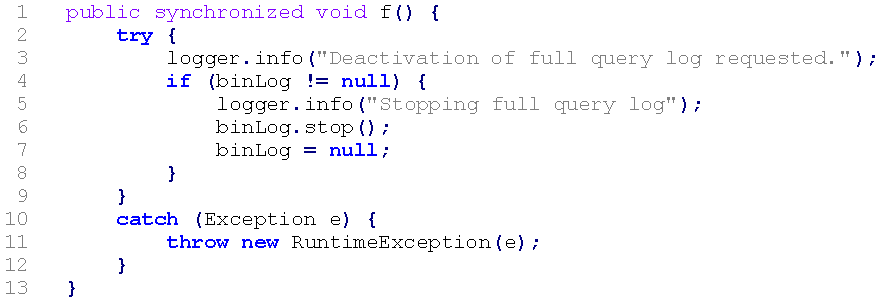
\includegraphics[width=0.82\linewidth]{stop.pdf}}
\hfill
\subfigure{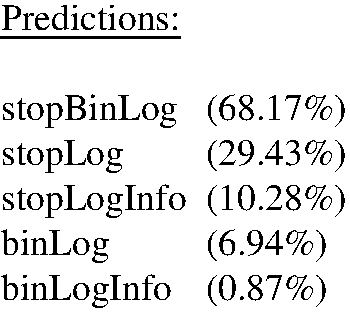
\includegraphics[width=0.17\linewidth]{prediction.pdf}}
\caption{示例代码段以及函数名预测}
\label{stop}
\end{figure}

\section{相关研究}
本节首先介绍了代码分布式表示模型,这些模型通过学习对代码的中间表示,将代码片段表示为难以直接解释的向
量。然后介绍了与代码属性预测模型,最后介绍了关于代码到自然语言的转换模型。

\subsection{代码表示模型}
在局部表示中,向量中的每个值通常有具体的明确的含义,例如在One-Hot表示模型中,当第$i$维数值为0时,表
示其对应的元素没有现在该样本中。与局部表示不同,分布式表示~\cite{hinton1984distributed}假设所表示的
元素可以在多维实数空间内进行编码,并且可以在该空间内评估两个表示之间的相关性。因此,分布式表示的结果
通常是一种矢量或矩阵,其元素的含义分布在多个维度上。由于具有较好的总结能力,分布式表示经常在自然语言
处理领域中被用来对自然语言中的元素进行编码。例如,Mikolov等人~\cite{mikolov2013efficient}通过学习自
然语言中单词的分布式表示,学到了单词之间的相关性。

由于在机器学习和自然语言处理上的成功运用,近年来,越来越多的研究者使用分布式表示模型表示代码,将代码
元素映射到矢量中。通过这样的方式,能够根据上下文学习代码的语义,具有相似上下文的代码通常具有相似的语
义。代码表示模型类似于自然语言处理中的文本表示模型,根据代码的表示代码表示模型可用来预测代码片段的属
性概率分布,如变量和函数名等。Mou等人~\cite{mou2016convolutional}使用自定义的卷积神经网络来学习代码
片段的分布式矢量表示,然他们混合了学生对各种课程问题的解决方案,通过分类来恢复这些解决方案到问题的映
射。Piech等人~\cite{piech2015learning}和Parisotto等人~\cite{parisotto2017neuro}学习了源代码输入/输出
对的分布式表示,并使用这些表示来评估和审查学生任务。除此以外,部分研究使用分布式表示来学习上下文信息
并生成代码。例如,Maddision等人~\cite{maddison2014structured}通过对上下文进行分布式表示,按序生成代
码。Ling等人~\cite{ling2016latent}和Allamanis等人~\cite{allamanis2015bimodal}将代码上下文分布式表示
与自然语言的分布式表示相结合来合成代码。Livshits等人~\cite{livshits2009merlin}通过分布式表示来解决信
息流问题。

\subsection{代码属性预测}
通过使用代码的抽象表示作为输入,得到关于代码属性在输入代码上的条件概率分布并进行预测代码的属性。
Allamanis等人~\cite{allamanis2014learning,allamanis2015suggesting,allamanis2016convolutional}发现变
量和函数名的分布式表示可以学到常见的语义属性,使用上下文信息学习变量和函数的分布式矢量表示,并使用这
种表示来预测变量名和函数名的概率分布。

Raychev等人~\cite{raychev2015predicting}将代码表示为变量依赖关系网络,将每个javaScript变量表示为一个
节点,并将其中的变量交互建模为条件随机场(CRF),最后通过联合预测代码片段中所有变量的类型和名称。受
统计机器翻译启发,Gu等人~\cite{gu2016deep}引入序列到序列的深度神经网络
~\cite{sutskever2014sequence},学习了自然语言查询的中间表示,并用来预测相关的API调用序列。Murali等人
~\cite{murali2017finding}利用主题模型的组合来学习一个循环神经网络,该神经网络为API调用序列建模。该模
型可来检测可能性极小的API调用序列,从而检测Android代码中实际存在的缺陷。除此以外,Allamanis等人
~\cite{allamanis2018learning}还通过学习将代码片段粘贴到现有的代码中,并调整所使用的变量来预测代码的
数据流图。Allamanis等人~\cite{allamanis2018learning}使用代码上下文中的各种元素来检测特定类型的缺陷,
如变量和操作符误用等。

\subsection{代码到自然语言的转换}
通过学习代码与自然语言文本的关系,可以自动生成代码文档,增加代码可读性。Oda等人
~\cite{oda2015learning}使用机器翻译技术将Python代码翻译成伪代码,从而生成易读性更高的代码;Iyer等人
~\cite{iyer2016summarizing}设计了一个将代码总结为文本的神经注意力模型。Movshovitz等人
~\cite{movshovitz2013natural}构建了一个推荐系统用来在给定源代码片段的情况下协助完成评论,该系统使用
类似主题的图模型来为上下文信息建模。

根据代码生成文本还可以用来自动生成注释。Sridhara等人~\cite{sridhara2010towards}提出了一种使用程序结
构信息为java函数生成摘要注释的方法,该方法的基本思想是从函数中选出重要的语句,然后将其翻译成自然语
言。该方法首先构建函数的数据流程图,然后分析该数据流来识别重要的语句。Wong等人
~\cite{wong2013autocomment}通过问答网站自动生成评论,从问题标题和回答文本中提取代码和描述的映射,并
使用代码克隆检测技术来查找与该映射相近的代码片段,查找出来的代码对通常是由开发人员从项目中复制的代
码,然后识别该代码片段的注释并重新应用于其他项目。然而,虽然这种方法可以应用于数百万个项目,但是其仅
对小部分代码片段有效,但无法为某个项目生成大量注释。

\section{研究方法}
本章提出了基于层次注意力的函数名推荐模型,该模型以编码-解码模型~\cite{Kyunghyun2014Learning}
(Encoder-Decoder)为基本框架,通过输出词项序列(Token Sequence)来为给定代码片段预测函数名。本节首
先简要阐述编码器-解码器的原理,然后介绍本章的模型架构,接下来依次介绍模型架构的各个组成部分,包括代
码片段的输入表示、编码器、解码器等;最后描述在预测阶段,针对给定的代码段,如何利用训练好的模型使用集
束搜索(Beam Search)生成具有概率的函数名列表。



\subsection{模型架构}


\subsubsection{编码-解码模型}
编码-解码模型为常见的一种模型框架,其核心思想是将输入$x$通过编码转化为一个向量$C$,再将向量$C$通过解
码转化为输出$y$。其中用来编码的模型为编码器(Encoder),用来解码的模型为解码器(Decoder)。编码器和
解器均可以为任意的模型;输入和输出也可以是任意的形式,如文字、图像等。当$x$和$y$均为序列时,这样的模
型也被称为序列到序列模型(Seq2Seq)。在实际应用中存在很多序列到序列的问题,例如翻译、问答系统等。

图~\ref{fig:seq2seq}为一个序列到序列模型的例子,其中编码器和解码器均使用循环神经网络(Recurrent Neural
Networks, 简称RNN)。给定输入序列$x=\{x_1,x_2,...,x_m\}$,该模型使用RNN将输入序列$x$编码为一个固定长
度的向量$C$,然后使用RNN将向量$c$解码为输出序列$y=\{y_1,y_2,...,y_n\}$,从而学习关于输出序列$y$在输
入序列$x$上的条件分布。在RNN中,第$t$个时刻的隐藏状态用$h_t$表示,该隐藏状态由前一个隐藏状态
$h_{t-1}$和第$t$个时刻的输入$x_t$共同决定:
\begin{eqnarray}
    h_t = f(h_{t-1},x_t),
\end{eqnarray}
因此,当输入完成时,当前隐藏状态$h_m$中包含了整个输入序列$x$的信息,通常将其作为输入序列$x$的编码
$C$。在解码阶段,同样使用RNN,以$C$作为输入,生成输出序列$y$,不同的是,生成$y_t$的概率还需要考虑已
经生成的输出$y_1,y_2...y_{t-1}$:
\begin{eqnarray}
    p(y_t|y_1,y_2,...,y_{t-1},C) = g(y_{t-1},H_t,C).
\end{eqnarray}
其中第$t$个时刻的隐藏状态$H_t$由前一个时刻的隐藏状态$H_{t-1}$和输出$y_{t-1}$以及输入的编码$C$共同决定:
\begin{eqnarray}
    H_t = f(H_{t-1},y_{t-1},C).
\end{eqnarray}
通过这样的方式,可以在输入序列的长度$m$和输出序列的长度$n$不相等的情况下,构建一个关于输出序列$y$在
输入序列$x$上的条件分布的生成模型$p(y_1,y_2,...,y_n|x_1,x_2,...,x_m)$,然后通过最大似然的方式拟合数
据集。

\begin{figure} [!t]
	\centering
	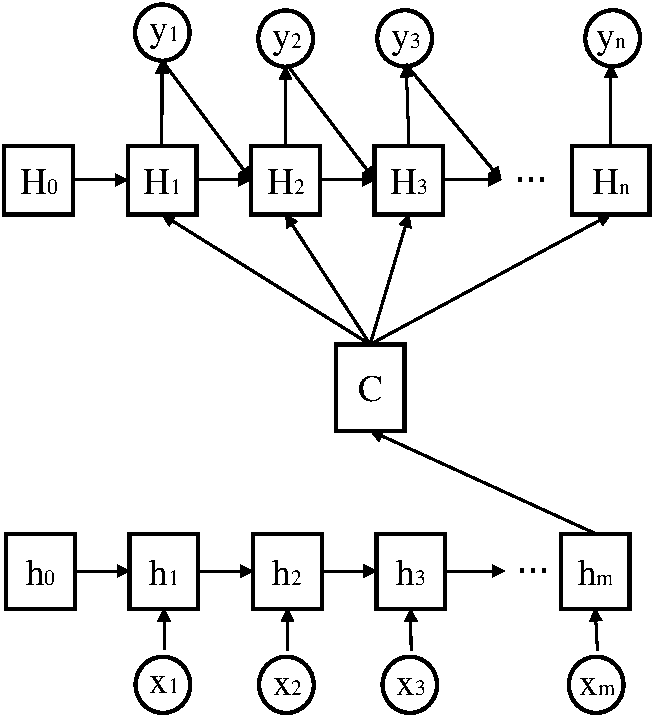
\includegraphics[width=0.45\textwidth]{seq2seq.pdf}
	\caption{RNN编码-解码模型}
	\label{fig:seq2seq}
\end{figure}

本章提出的基于层次注意力的函数名推荐模型,与上述模型有相似的架构,均为序列到序列的编码-解码模型。两
者的区别是,本文使用层次注意力作为编码器将代码段表示为固定长度的向量,然后使用GRU序列模型作为解码
器,通过学习函数名关于代码段的条件概率分布,输出构成函数名的词项序列(Token Sequence)。

\subsubsection{函数名推荐模型架构}
本章模型的架构如图~\ref{fig:arch}所示。可以看出,该模型为编码-解码模型
~\cite{Kyunghyun2014Learning}。为了提高模型的抽象和总结能力,本文使用程序分析将函数功能拆分为多个由
基本代码块组成的子功能,不同基本代码块对预测函数名的重要性不同;同时,一个代码块由多个词项组成,不同
的词项的重要性也不同。为了模拟这样的层次结构,在编码阶段引入层次注意力模型
~\cite{yang2016hierarchical}分别学习基本代码块和词条(token)对预测函数名的重要性,通过编码-解码模型
学习函数名在代码片段上的条件分布。

\begin{figure} [!t]
	\centering
	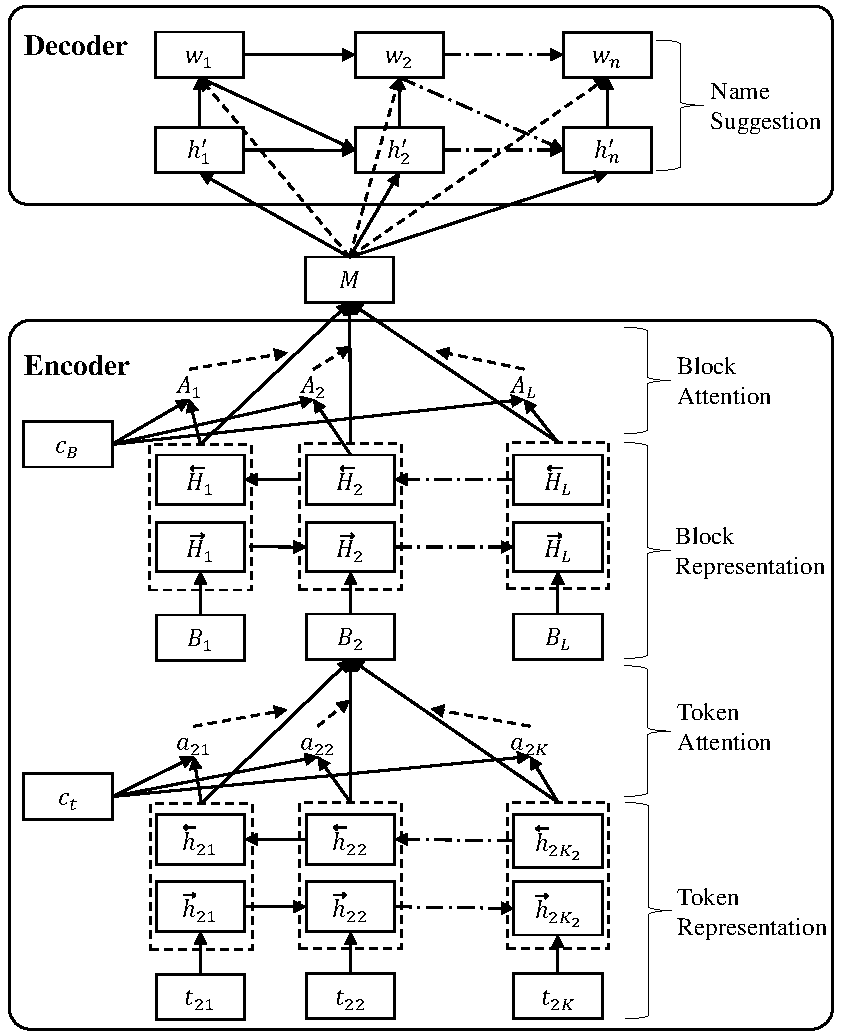
\includegraphics[width=0.65\textwidth]{architecture.pdf}
	\caption{基于层次注意力的函数名推荐模型架构}
	\label{fig:arch}
\end{figure}

如图~\ref{fig:arch}所示,编码器对代码片段的表示分为两个阶段:在第一阶段,给定输入的词项序列,学习基
本代码块的表示;在第二阶段,以基本代码块序列列作为输入,学习整个代码片段(函数体)的表示。 在解码阶
段,以代码片段的表示作为输入,使用门控循环单元~\cite{Kyunghyun2014Learning}模型学习组成函数名的词项
序列在代码片段上的条件分布。同样,在计算当前隐藏状态$h_t'$时考虑上一个时刻的输出$w_{t-1}$,使模型能
快速收敛。

基于层次注意力的函数名推荐模型,其输入是由基本代码块序列构成的代码片段,输出是由词项序列构成的函
数名。给定函数$m$,将其表示为由基本代码块组成的序列$m=(B_1,B_2, \dots, B_L)$,每个基本块由词项序列表
示,例如$B_2 = (t_{21}, \dots, t_{2K_2})$,其中$K_2$为基本代码块$B_2$中所包含的词项的个数。模型的输
出为词项序列$(w_1, \dots, w_n)$,表示预测的函数名。需要注意的是,输入和输出序列的长度可以不一致,事
实上,与代码的长度相比,函数名的长度通常非常短,因此为给定代码片段预测函数名的困难较大。

编码器首先根据输入的基本代码块序列,通过层次注意力将函数体表示为一个固定长度的向量$M$:
\begin{equation}
M = f({B_1, \dots, B_L}) \,.
\label{eq:encoder}
\end{equation}
然后解码器依次预测组成函数名的词项,根据上一个时刻的词项和解码器的输出向量$M$,预测当前时刻的词项:
\begin{equation}
P(w_j|\{w_1, \dots, w_{j-1}\}, M) = g(\{w_1, \dots, w_{j}\}, M) \,,
\label{eq:decoder}
\end{equation}
其中$g$的输出为一个概率,表示根据代码片段的表示向量$M$和上一个时刻的输出词项$w_{j-1}$,预测当前词项
为$w_j$的概率,本文使用softmax激活函数使函数$g$的输出为一个概率值。

将解码器和编码器联合起来,能够学习关于函数名的词项序列$w$在由词项组成的代码段$t$上的条件分布
$p(y|t)$,最后通过最大条件对数似然来优化该联合模型:
\begin{equation}
\max \limits_{\bm\theta} \frac{1}{N}\sum_{n=1}^{N} \log p_{\bm\theta}(\bm w_n | 
\bm t_n) \,,
\label{eq:loss}
\end{equation}
其中$N$表示训练样本的个数,$\bm\theta$为模型中的参数,通过使用随机梯度下降来优化模型的参数。

\subsection{输入代码段表示}
\label{represent}
为了提高模型的抽象和总结能力,本文将函数体拆分为多个基本代码块,每个代码块作为执行函数子功能的最小单
元,通过注意力机制学习不同基本代码块对函数名预测的重要性。

借鉴于程序指令中基本块的定义,本文将基本代码块定义如下:
\begin{Definition}
    基本代码块。基本代码块为顺序执行的代码语句,每个基本代码块有且只有一个入口和出口。
\end{Definition}

为了对函数体进行划分,首先根据函数的控制流信息将函数中的代码片段表示为如图
~\ref{block-example}所示的代码结构树。根据基本代码块的定义,每个基本代码块有且只有一
个入口,且基本块中的语句是顺序执行的,因此对基本代码块的划分主要依赖于对代码基本
块入口的寻找。给定函数$m$以及其代码结构树$Tree(m)$,通过遍历其代码结构树来寻找函
数体中的入口语句集合$E(m)$。算法~\ref{alg:block}描述了获取入口语句集合的遍历过
程。具体来说,首先对于函数$m$,其中第一条语句一定是入口语句,因此将其加入入口语
句集合中;通过宽度优先算法遍历函代码结构树$Tree(m)$,从左往右依次判断节点是否为
叶子节点;若该节点不是叶子节点,则访问下一个节点;若该节点是叶子节点,且其左兄弟
不是叶子节点,则将该节点对应的语句加入入口语句集合中;否则继续访问下一个节点。

在找到所有的入口语句后,对函数中代码片段的划分过程为:按照代码的顺序,从函数的第
一个入口语句开始,直到遇到下一个入口语句或是函数结束,为一个基本代码块。以图
~\ref{block-example}中的代码和代码结构树为例,按照算法~\ref{alg:block}可以得到入
口语句为$(S_2,S_4,S_6,S_9,S_{12},S_{16})$,因此根据上述过程可将示例函数划分为6个
基本代码块,每个基本代码块为顺序执行的代码语句。

\begin{algorithm}[H]
\caption{入口语句搜索算法}\label{alg:block}
\KwIn{函数$m$;}\\
\KwOut{入口语句集合$E(m)$;}\\
获取函数$m$的代码结构树$Tree(m)$;\\
将函数入口语句加入集合$E(m)$;\\
初始化所有节点的状态为未访问;\\
初始化队列$queue=\emptyset$;\\
将根节点压入队列queue;\\
\While {$queue \neq \emptyset$} {
    从队列中移除并返回头顶节点作为当前节点;\\
    \If {当前节点为叶节点} {
        \If {当前节点的左兄弟不是叶子节点且不在集合$E(m)$中} {
            将当前节点的对应语句加入集合$E(m)$;\\
        }
    }
    \Else{
        将当前节点的所有未被访问的子节点加入队列$queue$;\\
    }
    标记当前节点的状态为已访问;\\
}
\textbf{return} 入口语句集合$E(m)$。\\
\end{algorithm}

在将函数体进行划分后,得到基本代码块序列$m=\{B_1, \dots, B_L\}$,其中每个代码基
本块为一个词项序列$B_i=\{t_{i1},t_{i2},\dots,t_{iK_i}\}$。需要注意的是,由于函数体
中标识符的存在,因此对程序语言的分词除了根据非英文字符以外,本文对标识根据两种命
名惯例进行分词,分别是下划线命名法(如set\_params)和驼峰命名法(如setParams或
SetParams)。通过这样的方式,得函数体的层次结构表示作为模型的输入。


\subsection{基于层次注意力的编码器}
在编码阶段,本文采用层次注意力模型将给的那个代码片段表示为固定长度的向量。接
下来自底向上详细阐述本章模型中的编码器。

\subsubsection{门控循环单元}
基于层次注意力的函数名推荐模型,在编码器和解码器中都使用了门控循环单元
~\cite{Kyunghyun2014Learning}作为基础模型。门控循环单元(Gated Recurrent Unit,简称GRU)通过门控机制
处理远距离依赖,其效果与同样使用门控机制处理远距离依赖的长短期记忆模型~\cite{Hochreiter1997Long}
(Long Short-Term Memory,简称LSTM)相差不多,但由于GRU的参数较少,因此收敛速度较快,所需要的样本较
少~\cite{Chung2014Empirical}。

GRU模型的门控机制包括两个门计算,分别重置门和更新门。前者用于控制当前时刻的输入如何与上一个时刻的信
息相结合,后者用于控制上一个时刻的信息被保留到当前时刻的程度,通过这样的方式,GRU模型能够控制以前的
信息被保留和遗忘的程度,从而在一定程度上解决了RNN的梯度消失的问题。

\begin{figure} [!t]
	\centering
	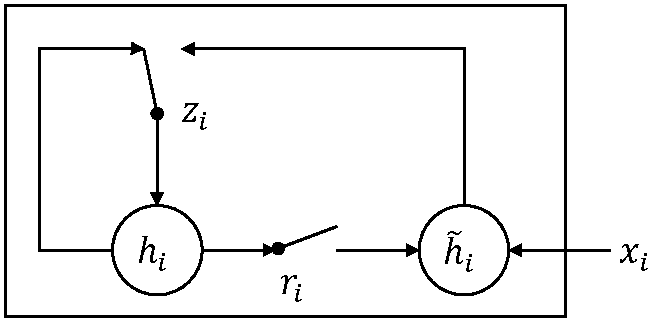
\includegraphics[width=0.35\textwidth]{gru.pdf}
	\caption{门控循环单元示意图}
	\label{fig:gru}
\end{figure}

图~\ref{fig:gru}为GRU模型的门控示意图,其中$z_s$和$r_s$分别表示第$s$个时刻的更新门和重置门。更新门$z_s$控制了过去信息和输入信息中需要被继续传递的部分,通过以下公式进行计算:
\begin{equation}
    z_s = \sigma (W_z x_s + U_z h_{s-1} + b_z) \,,
    \label{eq:gru_update}
\end{equation}
$x_s$为第$s$个时刻的输入向量,$h_{s-1}$为上一个时刻的隐藏状态,$W_z$和$U_z$为权重矩阵,$b_z$为偏差。
公式~\eqref{eq:gru_update}通过对$x_s$和$h_{s-1}$分别进行线性变换,再将这两部分信息相加并使用激活函数
得到更新门$z_s$,更新门的存在使模型能够有选择性地保留过去记忆和当前输入中的信息。

图~\ref{fig:gru}中的$r_s$为重置门,重置门根据过去记忆和当前输入,决定了过去记忆被忽略的程度。重置门
的计算公式与更新门类似,但参数不同:
\begin{equation}
    r_s = \sigma (W_r x_s + U_r h_{s-1} + b_r) \,,
    \label{eq:gru_ret}
\end{equation}
其中$W_r$和$U_r$为权重参数,$b_r$为偏差,$x_s$为当前的输入,$h_{s-1}$为上一个时刻的隐藏状态。

接下来阐述更新门$z_s$和重置门$r_s$是如何帮助模型有选择性地将过去的记忆与当前的输入相结合,并继续传递
的。首先根据重置门对过去记忆的存储选择,可以得到新的记忆内容:
\begin{equation}
    \tilde{h}_s = \tanh (W_h x_s + r_s \odot (U_h h_{s-1}) + b_h) \,,
    \label{eq:gru_cand}
\end{equation}
其中新的记忆内容由两部分组成,第一部分为输入信息$x_s$,第二部分为重置门$r_s$控制的过去记忆,重置门通
过Hadamard乘积控制过去记忆$h_{t-1}$被保留的程度,通过将这两部分信息相加,得到当前的新记忆内容
$\tilde{h}_s$。

最后通过更新门控制对当前记忆和过去记忆的传递程度,计算得到当前时刻的隐藏状态:
\begin{equation}
	h_s = (1-z_s) \odot h_{s-1} + z_s \odot \tilde{h}_s \,,
    \label{eq:gru_h}
\end{equation}
其中$z_s$为更新门,控制了当前记忆$\tilde{h}_s$和过去记忆$h_{s-1}$中需要传递的信息。更新门和重置门让
模型能够有选择的控制过去记忆的保留和传递,从而使得模型在能够捕捉长期依赖的前提下减少梯度消失。


\subsubsection{词项表示}
给定函数体$m=\{B_1,B_2,\dots,B_L\}$,其中的每个基本代码块都由词项表示。本章模型的主要任务是为给定函
数体预测函数名,因此首先要将函数体中的词项用向量表示。具体来说,首先针对给定训练数据集中的词项构建一
个字典,过滤掉频率过低的词项。对于函数体中的每个基本代码块$B_i=\{t_{i1},t_{i2},\dots,t_{iK_i}\}$,词
嵌入矩阵$W_e$将词项$t_{ij}$转化为向量$x_{ij}=W_e t_{ij}$,然后使用双向GRU模型学习基本代码块
的表示,对于每个输入词项$t_{ij}$,从两个方向获取其上下文信息。对于每个基本代码块$B_i$,前向
GRU从$t_{i1}$到$t_{iK_i}$读取词项,后向GRU从$t_{iK_i}$到$t_{i1}$读去词项:

\begin{align}
	x_{ij} &= W_e t_{ij} \quad\text{(Embedding)} \,, \\
	\overrightarrow{h}_{ij} &= \overrightarrow{GRU}(x_{ij}) 
	\quad\text{(Forward GRU)} \,, \\
       \overleftarrow{h}_{ij} &= \overleftarrow{GRU}(x_{ij}) 
       \quad\text{(Backward GRU)} \,, \\
       h_{ij} &= [\overrightarrow{h}_{ij}, \overleftarrow{h}_{ij}] 
       \quad\text{(Concatenation)} \,,
\label{eq:token_encoder}
\end{align}
其中$j\in [1, K_i] \cap N^+$。在从两个方向计算出词项的隐藏状态后,双向
GRU模型将这两个隐藏状态连接起来作为该词项的表示。需要注意的是,本文中
的词嵌入矩阵$W_e$并没有使用预训练好的词嵌入矩阵,而是通过高斯分布随机初始化
词嵌入矩阵$W_e$,该矩阵在训练过程中随模型的其它参数一起优化。根据双向GRU模型中的隐藏状
态,每个词项得到一个向量表示,该表示考虑了两个方向的上下文信息。

\subsubsection{词项注意力}
在函数$m$中,每个基本代码块由一个词项序列表示
$B_i=\{t_{i1},t_{i2},\dots,t_{iK_i}\}$,然而并不是每个词项对于基本代码块的表示都
具有同等的重要性。例如,在代码``int sum = len1 + len2;''中,词项``int''对于代码
功能的重要性大概率低于词项``sum''。因此,为了学习不同词项对基本代码块的重要性,
引入了注意力机制为每个词项分配一个权重:

\begin{align}
    u_{ij} &= c_t^\top \tanh(W_t h_{ij} + b_t) \,, \\
    a_{ij} &= \frac{\exp{u_{ij}}}{\sum_{j^\prime=1}^{K_i} \exp{u_{ij^\prime}}} 
    \,, \\
    B_{i} &= \sum_{j=1}^{K_i} a_{ij}h_{ij} \,,
\label{eq:token_attn}
\end{align}
其中$j\in [1, K_i] \cap N^+$,$c_t$为词项级别的上下文向量表示,在训练
中与其它参数一起学习,$W_t$表示词项的权重参数,$b_t$为偏差,并使用Softmax函数将权重规则化。最
后,每个基本代码块通过组成该基本块的词项的权重和来表示。

\subsubsection{基本代码块表示}
在表示基本代码块时,同样考虑了基本代码块的上下文信息,因此使用类似的双向GRU模型
来获取其上下文信息。给定函数$m$,将其通过基本代码块序列表示,即$M = (B_1, \dots,
B_L)$,每个基本代码块$B_i$的隐藏状态为:
\begin{align}
    \overrightarrow{H}_i &= \overrightarrow{GRU}(B_{i}) 
\quad\text{(前向GRU)} \,, \\
    \overleftarrow{H}_i &= \overleftarrow{GRU}(B_i) 
\quad\text{(后向GRU)} \,, \\
    H_i &= [\overrightarrow{H}_i, \overleftarrow{H}_i] 
\quad\text{(连接)} \,,
\label{eq:block_encoder}
\end{align}
其中$i\in [1, L] \cap N^+$。双向GRU模型通过从两个方向来表示基本代码块$B_i$的上下
文信息,通过这种方式,同样可以得到每个基本代码块的隐藏状态表示。

\subsubsection{基本代码块注意力}
本文将函数体表示为由基本代码块组成的序列,虽然本文假设每个基本代码块完成函数的一
个子功能,但不同基本块完成的子功能不同,其对函数整体功能的影响也不同。为了让模型
能够学到不同基本代码块对函数名预测的重要性,在使用基本代码块表示函数体时,再次引
入了注意力机制,为每个基本代码块分配不同的权重。用$c_B$表示每个基本代码块对预测
函数名的重要性,可以得到:

\begin{align}
v_i &= c_B^\top \tanh(W_B H_i + b_B) \,, \\
A_i &= \frac{\exp{v_i}}{\sum_{i^\prime=1}^{L} \exp{v_{i^\prime}}} 
\,, \\
M &= \sum_{i=1}^{L} A_i H_i \,,
\label{eq:block_attn}
\end{align}
其中$i\in [1, L] \cap N^+$,$c_B$在随机初始化后,通过优化模型得到;$W_B$是基本代码块的权重参数,$b_B$
为其对应的偏差。最后函数体的表示向量$M$通过基本代码块的权重和得到。通过这样的方式,表示向量$M$通过层
次的方式对整个函数的信息进行编码,在编码时考虑了不同词项对基本代码块表示的重要性可能不同,也考虑了不
同基本代码块对函数表示的重要性可能不同,并在接下来的解码器中作为输入预测组成函数名的词项序列。

\subsection{基于门控循环单元模型的解码器}
为了预测函数名,在解码阶段使用另一个GRU模型将通过编码器得到的函数表示$M$转化为词项序列
$\{y_1,y_2,...,y_K\}$。如公式~\eqref{eq:decoder}所示,在第$k$个时刻,输出为$y_k$的概率与函数在解码器
中的编码$M$和前面已经生成的输出$y_1,y_2,...,y_{k-1}$相关。需要注意的是,由于理论上函数名与代码片段不
在同一个空间,因此函数名中的词项$y$与输入代码段中的词项$t$具有不同的表示,即词项$y_k = W_w w_k$,其
中$W_w$为另一个词嵌入矩阵。

为了表示在解码器中,第$k$个时刻的输入为上一个时刻的输出$y_{k-1}$和函数表示$M$,将公式
~\eqref{eq:gru_update}--\eqref{eq:gru_h}中关于GRU模型的计算过程稍作修改,增加了函数表示$M$作为输入:
\begin{align}
z_k &= \sigma(W_z y_k + U_z h^\prime_{k-1} + \underline{V_z M} + b_z) \,, \\
r_k &= \sigma(W_r y_k + U_r h^\prime_{k-1} + \underline{V_r M} + b_r) \,.\\
\tilde{h}^\prime &= \tanh(W_h y_k + r_k \odot (U_h h^\prime_{k-1}) + 
\underline{V_h M} + 
b_h) \,, \\
h^\prime_k &= (1-z_k)\odot h^\prime_{k-1} + z_k \odot \tilde h^\prime_k \,, 
\end{align}
其中增加函数表示$M$作为输入的部分用下划线标记出来,$V_{*}$为增加的输入向量$M$的权重参数。同样使用更
新门和重置门控制对过去记忆$h^\prime_{k-1}$的保留和遗忘。在得到第$k$个时刻的隐藏状态$h^\prime_k$后,
使用Softmax激活函数来预测第$k$个时刻输出词项为$y_k$的概率:
\begin{align}
p(y_k&|\{y_{k-1}, \dots, y_1\}, M) \notag\\
&= \text{softmax}(W_o(y_{k-1} + W_{h^\prime}h^\prime_k + W_M M) + b_o) \,,
\label{softmax}
\end{align}
其中$W_o$、$W_{h^\prime}$和$W_M$为Softmax层的参数,$b_o$为偏差。公式~\eqref{softmax}在计算第$k$个时刻
输出为$y_k$的概率时,将$y_{k-1}$作为和函数的表示向量$M$作为输入,通过这种强制教导(Teacher
Force~\cite{Williams1989learning})的方式提高模型训练的效率。

\subsection{集束搜索函数名推荐}
在测试阶段,给定输入函数体$m$,通过在每个时刻选择概率最大的词项作为输出,直到输出结束符号为止,能够
得到一个词项序列$\{y_1,y_2,\dots,y_m\}$。将输出的词项序列按照命名惯例组合起来,则得到为给定函数体$m$
预测的函数名。然而,这种生成方式只能预测一个函数名。为了尽可能接近最优解,本文通过在预测阶段使用集束
搜索(Beam Search),为给定函数体生成一个函数名列表,从而扩大用户的选择范围。

集束搜索为序列到序列模型中常用的启发式搜索方式~\cite{Graves2012Sequence,sutskever2014sequence},这种
搜索方式在本质上基于贪心思想,但由于其扩大了搜索范围,因此能够得到更多的解。假设集束宽度为2,在第一
个时刻选择概率最大的两个词项$y_{11}$和$y_{12}$,将$y_{11}$和$y_{12}$分别当作第一个时刻的词项$y_1$,
通过公式~\eqref{softmax}得到在给定$y_1$的情况下词项$y_2$的条件概率$p(y_2|y_1,m)$,根据公式
~\eqref{beam}可以得到给定输入函数体$m$时,输出词项序列为$y_1,y_2$的概率。选择概率最大的两个词项序
列,重复上述的过程,直到遇到结束符号位置。通过这样的方式,可以为给定函数体$m$生成具有概率的函数名候
选集。
\begin{align}
p(y_2,y_1|m) = p(y_2|y_1,m)p(y_1|m) \,,
\label{beam}
\end{align}

\section{实验设计}
本节评估了基于层次注意力的函数名推荐模型的有效性,通过在10个开源软件系统上进行实
验,对比评估了基于层次注意力的模型与其它三种模型推荐函数名的准确性,验证了本章方
法的有效性。

\subsection{实验对象与数据处理}
本章的实验对象为10个来自GitHub的开源软件系统。表~\ref{benchmark3}为实验对象的统
计数据,可以看出,本章的实验对象为GitHub上收藏和使用较多的开源软件系统,且规模较
大。由于大规模软件系统的维护成本和维护难度较高,因此提高大型软件系统的易读性和维
护效率具有重要的意义。


为了根据不同软件系统的代码习惯推荐个性化的函数名,同时与之前的研究保持一致,在实
验中针对每个软件系统训单独训练一个函数名推荐模型。具体来说,对于表
~\ref{benchmark3}中的每个软件系统,首先提取其中所有的函数,并过滤掉其中的抽象函
数、构造函数和重写函数。过滤掉抽象函数是因为模型的输入为构成函数体的代码
片段,而抽象函数没有代码片段,无法正常预测;过滤掉构造函数是因为构造函数的函数名
与类名相一致,因此对函数名的推荐类似于推荐类名称,与本文模型的主要目的不同;过滤
掉重写函数是因为重写函数由于重复的原因,在模型中很容易预测。
通过这样的方式,针对每个软件系统能够获得一个函数样本集,将样本集随机打乱,并将其
中80\%的样本作为训练数据,10\%的样本作为验证数据,剩下的10\%作为测试数据来评估模
型在该软件系统上的有效性。

\begin{table}[!t]
\zihaowu
\renewcommand{\arraystretch}{1.4}
% if using array.sty, it might be a good idea to tweak the value of
% \extrarowheight as needed to properly center the text within the cells
\caption{实验对象统计数据}
\label{benchmark3}
\centering
\begin{tabular}{l@{\quad}l@{\quad}l@{\quad}l@{\quad}l}
\toprule 
软件名称 &规模(M) &函数数量 &收藏数量 &使用数量\\ 
\midrule
Apache Cassandra &11.1 &10,466 &4,502 &2,061\\ 
Elasticsearch &19.8 &15,409 &32,393 &11,104\\ 
Gradle &14.1 &16,050 &7,096 &2,227\\ 
Hadoop-common &37.5 &33,237 &121 &141\\ 
Hibernate-orm &21.6 &34,307 &3,275 &2,250\\ 
Intellij-community &5.84 &6,972 &6,182 &2,362\\ 
Liferay-portal &47.9 &52,539 &1,258 &2,114\\ 
Presto &11.0 &10,672 &7,755 &2,616\\ 
Spring-framework &29.3 &33,157 &22,182 &14,313\\ 
Wildfly &14.2 &9,566 &2,012 &1,805\\ 
\bottomrule
\end{tabular}
\end{table}

对于数据集中的每个函数,将其作为一个样本,函数体是为样本的输入代码段,函数为样本
的标签。对于除本章方法以外的三个模型,通过分词的方式将函数体和函数名进行表示为词
项序列,对于代码中与函数名相同的标识符,使用词项``SELF''进行代替,其余标识符则根
据两种命名惯例进行分词,分别是下划线式(my\_case)与驼峰式(myCase或MyCase),从
而得到样本的输入序列和输出序列。在评估本章模型时,需要将输入序列表示为具有层次结
构的词项和基本代码块序列。最后,利用训练集对模型进行训练,并通过验证集调整超参,
例如基本代码块中词项序列的最大长度、隐藏单元的个数等,并在测试集上评估方
法的有效性。为了使实验具有可重复性,已将本次实验的数据集发布。

\subsection{对比实验}
为了评估本章方法的有效性,将其与词频-逆文件频率算法、循环神经网络和卷积神经网络三个模型进行对比实
验。其中,词频-逆文件频率算法(Term Frequency–Inverse Document Frequency,简称tf-idf算法)为信息检索
领域常用的一种统计方法,其核心思想通过对比词项在文档中出现的频率与词项在数据库中出现的频率来判断词项
的重要性。在本章实验中,由于在构建词项字典时已经统计了每个词项在所有函数体中出现的频率,因此使用
tf-idf算法为给定函数体推荐函数名,只需要统计输入词项序列中每个词项在输入中出现的频率即可。由于函数名
推荐的本质是对函数功能的翻译和总结,因此本章还使用了在机器翻译领域有较好表现的双向RNN-attention模型
~\cite{bahdanau2015neural},该模型在双向RNN的基础上加入了注意力机制,被认为可以学习输入序列与输出序
列之间的权重关系。除此以外,本章还将基于层次注意力的函数名推荐模型与基于卷积神经网络和注意力机制的函
数名推荐模型~\cite{allamanis2016convolutional}(以下简称为CNN-attention模型)进行对比,该方法通过卷
积神经网络学习代码结构的局部特征。与该方法不同的是,本文将程序分析与注意力机制相结合,将函数拆分为多
个基本代码块,并学习每个基本代码块对函数名的重要性。最后,在训练阶段,使用推荐的参数对RNN-attention
和CNN-attention模型进行训练。在训练基于层次注意力的模型时,使用Adam梯度下降算法
~\cite{kingma2014adam}作为优化器,并使用了dropout~\cite{srivastava2014dropout}来防止模型过拟合。

\subsection{评估方法}
本章从函数名和词项两个角度评估函数名推荐模型的准确性。其中,函数名的匹配被定义为从开始符号起到第一个
结束符号为止,预测的词项序列与代表函数名的词项序列完全一致。而词项级别的评估方法则以词项为单位,不考
虑词项的顺序,只考虑词项的准确率、召回率和F值。具体来说,准确率表示预测的词项中正确预测的词项所占的
百分比;召回率表示函数名的词项序列中被成功预测到的词项所占的百分比;如公式~\ref{f1}所示,F值为这两者
的加权调和平均。需要注意的是,虽然通过集束搜索能够得到多个解,在实验中为每种模型只选择概率最高的解作
为该模型的最终预测结果。

\section{实验结果与分析}
本节从函数名与词项两个角度比较了基于层次注意力的函数名推荐方法与其它三种较为流行
的模型在函数名推荐任务上的表现。

\subsection{函数名推荐方法比较}
表~\ref{accuracy3}为函数名的匹配率比较,即对测试样本进行预测时,预测结果与样本中
的函数名完全一致的函数占总数的百分比。第一列为实验中所使用的模型,从上至下依次代
表tf-idf算法、基于循环神经网络与注意力机制的模型~\cite{bahdanau2015neural}(表中
简写为RNN)、基于卷积神经网络与注意力机制的函数名推荐模型
~\cite{allamanis2016convolutional}(简写为CNN)以及本章提出的基于层次注意力的模
型(简写为HIER)。表~\ref{accuracy3}中使用黑体表示被标记的数值具有明显优势,而同
一列中的两个黑体数值之间则没有明显的区别(+/-0.5\%以内)。

\begin{table}[!t]
\scriptsize
\renewcommand{\arraystretch}{1.3}
\caption{匹配率比较}
\label{accuracy3}
\centering
\begin{tabular}{ccccccccccc}
\toprule
方法 &Cassandra &Elasticsearch &Gradle &Hadoop &Hibernate &Intellij &Liferay &Presto &Spring &Wildfly\\ 
\midrule
TF-IDF&30.4\%&13.7\% &15.6\% &21.9\%&47.3\% &11.4\% &53.2\% &25.6\% &\bf{23.1\%} &22.9\%\\ 
RNN&23.9\% &8.9\% &12.0\%  &13.4\% &51.1\% &5.7\% &48.1\% &18.3\% &15.4\% &19.2\%\\ 
CNN& 27.6\% &17.5\% &19.3\% & 22.5\% &58.9\% &\bf{13.4\%} &59.2\% &23.8\% &21.9\% &\bf{23.6\%}\\ 
HIER&\bf{31.7\%} &\bf{18.3\%} &\bf{20.6\%} &\bf{24.1\%} &\bf{62.0\%} &12.8\% &\bf{63.7\%} &\bf{26.1\%} &\bf{23.5\%} &\bf{23.7\%}\\
\bottomrule
\end{tabular}
\end{table}

从表~\ref{accuracy3}可以看到,除了Hibernate和Liferay,四个模型在其它所有数据集上
的匹配率均不高(在5.7\%\textasciitilde31.7\%之间),表明了函数名预测任务存在一定
的难度。不难发现,在其中9个数据集上基于层次注意力的模型的匹配率高于或等于其它三
种模型,证明了该模型在函数名预测任务上的有效性。CNN模型取得了仅次于本文模型的匹
配率,而tf-idf和RNN模型的匹配率则相对较低。对于这样的实验结果,一个可能的原因是
CNN模型~\cite{allamanis2016convolutional}与本章模型都是针对函数名预测任务而提出
的,并在模型中通过不同的方式考虑了代码的结构信息;而tf-idf与RNN模型
~\cite{bahdanau2015neural}是针对文档提出的,因此在模型中没有考虑代码的结构信息。
除此以外,通过观察成功预测的函数名,发现大多数匹配的函数名所包含的词项较少,说明
对长函数名预测的难度更大。

\begin{table}  
\scriptsize
\caption{词项级准确性比较}  
\label{token-accuracy}
\centering  
\subtable[词项级准确率]{ 
\begin{tabular}{ccccccccccc}
\toprule
方法 &Cassandra &Elasticsearch &Gradle &Hadoop &Hibernate &Intellij &Liferay &Presto &Spring &Wildfly\\ 
\midrule
TF-IDF&41.7\% &31.4\% &34.9\% &40.4\% &47.3\% &33.1\% &64.9\% &50.3\% &38.1\% &48.8\%\\ 
RNN   &38.2\% &29.9\% &30.6\% &31.1\% &47.2\% &23.8\% &58.4\% &41.6\% &33.3\% &36.5\%\\ 
CNN   &50.4\% &34.7\% &\bf{40.9\%} &\bf{41.3\%} &62.4\% &\bf{35.1\%} &66.7\% &\bf{51.6\%} &37.6\% &48.9\%\\ 
HIER  &\bf{51.6\%} &\bf{35.4\%} &\bf{41.4\%} &\bf{41.5\%} &\bf{64.8\%} &34.2\% &\bf{69.3\%} &\bf{52.1\%} &\bf{42.0\%} &\bf{49.6\%}\\
\bottomrule
\end{tabular} 
\label{tab1}  
}  \\
 
\subtable[词项级召回率]{          
\begin{tabular}{ccccccccccc}
\toprule
方法 &Cassandra &Elasticsearch &Gradle &Hadoop &Hibernate &Intellij &Liferay &Presto &Spring &Wildfly\\ 
\midrule
TF-IDF&41.9\% &28.5\% &31.4\% &35.3\% &55.2\% &28.4\% &63.7\% &44.0\% &39.7\% &45.2\%\\ 
RNN   &35.1\% &21.8\% &25.3\% &26.7\% &54.5\% &21.2\% &55.1\% &37.9\% &30.6\% &29.7\%\\ 
CNN   &48.1\% &\bf{33.5\%} &35.3\% &\bf{39.2\%} &59.7\% &\bf{32.0\%} &\bf{67.8\%} &\bf{47.1\%} &39.5\% &45.1\%\\ 
HIER  &\bf{50.4\%} &32.9\% &\bf{36.9\%} &\bf{38.9\%} &\bf{63.8\%} &30.1\% &\bf{68.2\%} &\bf{47.4\%} &\bf{41.3\%} &\bf{47.1\%}\\
\bottomrule
\end{tabular}
\label{tab2}  
}  


\subtable[词项级F值]{          
\begin{tabular}{ccccccccccc}
\toprule
方法 &Cassandra &Elasticsearch &Gradle &Hadoop &Hibernate &Intellij &Liferay &Presto &Spring &Wildfly\\ 
\midrule
TF-IDF&41.8\% &29.9\% &33.1\% &37.9\% &54.6\% &30.6\% &63.9\% &46.9\% &38.4\% &46.9\%\\ 
RNN   &36.6\% &25.2\% &27.7\% &28.7\% &50.6\% &22.4\% &56.7\% &39.7\% &31.9\% &32.8\%\\
CNN   &49.2\% &\bf{34.1\%} &37.9\% &\bf{40.2\%} &61.0\% &\bf{33.9\%} &67.2\% &\bf{49.2\%} &38.5\% &46.9\%\\
HIER  &\bf{51.0\%} &\bf{34.1\%} &\bf{39.0\%} &\bf{40.1\%} &\bf{64.3\%} &32.0\% &\bf{68.7\%} &\bf{49.6\%} &\bf{41.6\%} &\bf{48.5\%}\\
\bottomrule
\end{tabular}
\label{tab3}  
}
\end{table} 

由于完全匹配两个序列的难度较高,为了比较预测结果与函数名的相似性,在实验中统计了
正确预测词项的情况来评估预测结果是否与函数名具有相似的语义。表
~\ref{token-accuracy}列出了四种模型在数据集上的词项级准确率、召回率和F值。可以看
到,词项级的准确率和召回率比匹配率明显更高,说明在某些情况下,虽然模型没有正
确预测给定代码片段的函数名,但仍然学到了部分的语义。同样,在表
~\ref{token-accuracy}中用黑体标记了每列中最大的一个或多个数值。可以发现,39个最
大数值中的26个数值为层次注意力模型的预测结果,13个为CNN模型的预测结果,证明了本
文方法能够在一定程度上预测出能够表达函数功能的关键词项;同时也反映了在编码阶段通
过层次注意力网络对代码片段的表示能够获得有效的代码语义信息。除此以外,tf-idf相比
较RNN模型取得了更好的结果,一个可能的解释是函数名中存在很大部分的词项来自于其对
应的函数体,且在该函数体中出现的频率高于在其他函数中出现的频率。

\subsection{操作符对模型的影响}
程序语言通常包括关键字、标识符、操作符以及其它特殊符号组成,为了评估程序语言中的
操作符对代码片段表示的影响,本文设计了一组对比试验,通过改变所有数据集的预处理方
式,评估模型是否能够学到操作符等特殊符号中所包含的语义。例如,是否能根据操作符学
习到与函数功能相关的语义。

具体来说,本节通过在数据预处理阶段采取不同的处理方式,得到两组不同的数据集,其中
一组训练数据、验证数据和测试数据中均不存在操作符,另一个为原来的数据集。表
~\ref{operator}为在四个模型上使用上述两组数据集得到的在所有软件上的平均匹配率、
词项准确率、词项召回率和词项F值。其中在包含操作符的数据集上进行实验的结果用
$w/i$表示,在不包含操作符的数据集上实验的结果用$w/o$表示。根据表~\ref{operator}
中的结果,可以发现从整体上看在两组数据集上的结果并没有很大的区别,说明当前这四种
模型主要通过关键词和标识符学习代码片段与函数明的语义关系。

\begin{table}[!t]
\zihaowu
\renewcommand{\arraystretch}{1.4}
\caption{不同与处理方式的比较}
\label{operator}
\centering
\begin{tabular}{cccccccc}
\toprule
 方法 &预处理方式 &匹配率 &词项准确率 &词项召回率 &F值\\ 
\midrule
\multirow{2}{*}{TF-IDF}&w/i&29.9\%&42.3\% &43.6\% &41.8\% \\ 
&w/o&29.3\% &41.9\% &44.1\% &41.4\% \\ 
\multirow{2}{*}{RNN}&w/i&19.3\% &37.1\% &36.0\%  &35.4\% \\ 
&w/o&18.7\% &37.3\% &36.5\% &35.8\% \\
\multirow{2}{*}{CNN}&w/i& 27.7\% &60.4\% &41.3\% &44.9\% \\ 
&w/o&26.3\% &60.2\% &37.1\% &43.6\% \\
\multirow{2}{*}{HIER}&w/i&30.1\% &57.1\% &44.7\% &46.2\% \\
&w/o&29.8\% &57.3\% &42.2\% &45.8\% \\
\bottomrule
\end{tabular}
\end{table}

\section{讨论}




\begin{table}[!t]
\scriptsize
\renewcommand{\arraystretch}{1.3}
% if using array.sty, it might be a good idea to tweak the value of
% \extrarowheight as needed to properly center the text within the cells
\caption{基于层次注意力的函数命名样例}
\label{samples}
\centering
\begin{tabular}{l||l} 
\toprule
函数 \& 预测结果 &函数 \& 预测结果 \\
\midrule
\tabincell{l}{
      %\includegraphics[scale=0.7]{1.pdf}
      {\color{blue}{public}} ByteBuffer \textbf{getIndexedValue}() \{\\
 \quad {\color{blue}{return}} clustering.get(indexedColumn.position());\\
    \}}
&\tabincell{l}{
      %\includegraphics[scale=0.7]{1.pdf}
      {\color{blue}{public boolean}} \textbf{isDataPresent}() \{\\
 \quad {\color{blue}{return}} !responses.isEmpty();\\
    \}}\\ 
 \tabincell{l}{\underline{Predictions}: \\getPositionValue (38.67\%), 
    getPosition (22.64\%), \\getIndex (15.21\%), get (3.87\%), column (1.36\%).}&
 \tabincell{l}{\underline{Predictions}: \\isEmpty (32.14\%),
    empty (17.41\%), responses (5.46\%), \\getResponses (3.61\%).}\\
 \hline
 \tabincell{l}{
      %\includegraphics[scale=0.7]{1.pdf}
      {\color{blue}{public long}} \textbf{getRepairedAt}() \{\\
 \quad {\color{blue}{return}} sstableMetadata.repairedAt;\\
    \}}
&\tabincell{l}{
      %\includegraphics[scale=0.7]{1.pdf}
      {\color{blue}{int}} \textbf{getHeartBeatVersion}() \{\\
 \quad {\color{blue}{return}} version;\\
    \}}\\ 
\tabincell{l}{\underline{Predictions}: \\getMinRepairedAt (24.91\%), 
    getRepairedAt (20.07\%), \\metadata (9.54\%), getMetadata (5.48\%), sstable (1.48\%).}&
\tabincell{l}{\underline{Predictions}: \\getVersion (42.47\%),
    version (18.07\%), get (2.87\%).}\\
\hline
 \tabincell{l}{
      %\includegraphics[scale=0.7]{1.pdf}
      {\color{blue}{public boolean}} \textbf{isClean}() \{\\
 \quad {\color{blue}{return}} partitions.isEmpty();\\
    \}}
&\tabincell{l}{
      %\includegraphics[scale=0.7]{1.pdf}
      {\color{blue}{private void}} \textbf{notifyCreateKeyspace}(...) \{\\
 \quad changeListeners.forEach(l -> l.onCreateKeyspace());\\
    \}}\\ 
\tabincell{l}{\underline{Predictions}: \\isEmpty (29.91\%), partition (15.32\%), \\empty (9.62\%), getPartition (3.15\%), clean (1.23\%).}&
\tabincell{l}{\underline{Predictions}: \\notifyNewKeyspace (38.25\%), createKeyspace (16.21\%), \\notifyKeyspace (12.54\%), keyspace (9.32\%).}\\
 \hline
\tabincell{l}{
      %\includegraphics[scale=0.7]{1.pdf}
      {\color{blue}{public static}} BoostingQueryBuilder \textbf{boostingQuery}() \{\\
 \quad {\color{blue}{return new}} BoostingQueryBuilder(positiveQuery);\\
    \}}
&\tabincell{l}{
      %\includegraphics[scale=0.7]{1.pdf}
      {\color{blue}{public}} BigArrays \textbf{getBigArrays}() \{\\
 \quad {\color{blue}{return}} bigArrays;\\
    \}}\\ 
\tabincell{l}{\underline{Predictions}: \\addQuery (36.13\%), 
    buildQuery (24.73\%), \\boostingQuery (14.22\%), query (3.41\%), build (1.62\%).}&
\tabincell{l}{\underline{Predictions}: \\getBigArrays (51.23\%),
    bigArrays (24.75\%), \\getArray (14.02\%), array (1.25\%).}\\   
 \hline
\tabincell{l}{
      %\includegraphics[scale=0.7]{1.pdf}
      {\color{blue}{public}} ByteSizeValue \textbf{getBufferSize}() \{\\
 \quad {\color{blue}{return}} bufferSize;\\
    \}}
&\tabincell{l}{
      %\includegraphics[scale=0.7]{1.pdf}
      {\color{blue}{void}} \textbf{setBackPressureEnabled}(...) \{\\
 \quad conf.back\_pressure\_enabled = backPressureEnabled;\\
    \}}\\ 
\tabincell{l}{\underline{Predictions}: \\getBufferSize (26.83\%), 
    bufferSize (15.58\%), \\getSize (9.81\%), sizeOf (1.78\%).}&
\tabincell{l}{\underline{Predictions}: \\setBackPressureEnabled (34.63\%), set (15.41\%) \\
 BackPressureEnabled (10.34\%), enable (5.67\%).}\\      
 \hline
\tabincell{l}{
      %\includegraphics[scale=0.7]{1.pdf}
      {\color{blue}{public static}} RecoveryStats \textbf{readRecoveryStats}(...) \{\\
 \quad RecoveryStats stats = {\color{blue}{new}} RecoveryStats(); \\
 \quad stats.readFrom(in);\\
 \quad {\color{blue}{return}} stats;\\
    \}}
&\tabincell{l}{
      %\includegraphics[scale=0.7]{1.pdf}
      {\color{blue}{protected}} BulkByScrollResponse \textbf{buildResponse}() \{\\
 \quad {\color{blue}{return new}} BulkByScrollResponse(took, task.getStatus(),\\
  \quad \quad \quad \quad \quad \quad indexingFailures, searchFailures, timedOut);\\
    \}}\\ 
\tabincell{l}{\underline{Predictions}: \\readFromStats (22.63\%), 
    getStats (12.21\%), \\createRecoveryStats (4.36\%), RecoveryStats (1.07\%).}&
\tabincell{l}{\underline{Predictions}: \\newResponse (16.72\%),
    createResponse (10.63\%), \\BulkByScrollResponse (9.23\%), index (0.46\%).}\\      
 \hline
\tabincell{l}{
      %\includegraphics[scale=0.7]{1.pdf}
      {\color{blue}{public static}} UUID \textbf{maxTimeUUID}({\color{blue}{long}} timestamp) \{\\
 \quad {\color{blue}{long}} uuidTstamp = fromUnixTimestamp(timestamp) - 1;\\
 \quad {\color{blue}{return new}} UUID(createTime(uuidTstamp), \\
 \quad \quad \quad \quad \quad \quad \quad MAX\_CLOCK\_SEQ\_AND\_NODE);\\
    \}}
&\tabincell{l}{
      %\includegraphics[scale=0.7]{1.pdf}
      {\color{blue}{public}} ColumnMetadata \textbf{getDroppedColumn}(...) \{\\
 \quad DroppedColumn dropped = droppedColumns.get(name); \\
 \quad {\color{blue}{return}} dropped == {\color{blue}{null}} ? {\color{blue}{null}} : dropped.column;\\
    \}}\\ 
\tabincell{l}{\underline{Predictions}: \\getTimeUUID (32.93\%), 
    getUUID (10.13\%), \\createTime (5.26\%), maxUUID (4.39\%), timestamp (0.36\%).}&
\tabincell{l}{\underline{Predictions}: \\getDroppedColumn (26.02\%), compareDropped (13.31\%), \\getName (8.24\%),
    dropped (17.27\%), column (10.89\%).}\\        

\bottomrule
\end{tabular}
\end{table}

为了直观基于层次注意力的函数名推荐模型是如何为给定代码片段推荐函数的,表~\ref{samples}列举了一些来自
Cassandra和Elasticsearch的函数。以每个函数的函数体作为输入代码片段,并使用集束搜索得到最多5个词项序
列作为推荐的函数名列表,并按照概率大小排序。需要注意的是,由于本文模型的输入并不包括函数的参数,因此
为了简洁,列举的函数中省略了函数本身的参数。

从表~\ref{samples}中可以看出,对于一些简单的函数,例如对于$getBufferSize()$和
$getBigArrays()$函数,模型能够很容易地预测出准确的函数名。通过分析实验中的预测结
果,发现模型能够较为准确地识别简单的$get$和$set$类型的函数,然后通过$(get|set)+
variable$的模式对函数名进行预测。这种方法在很多情况下能够正确预测函数名,但有时
也会与真实的函数名不一致。例如表~\ref{samples}中的$getHeartBeatVersion()$函数,
模型预测结果为$getVersion()$。

通过观察表~\ref{samples}中的$isDataPresent()$和$isClean()$函数,可以发现,这两个
函数的代码段有相似之处,即都使用$isEmpty()$函数判断变量是否为空。虽然这两个函数
中的变量名不同,但由于模型在预测时为它们的共同词项$is$和$empty$分配了较大的权
重,使得这两个函数具有相似的表示,从而得到相同的预测结果。

最后本文通过实验发现,由于函数命名存在一定的主观性,而目前的评估方法很难准确评估
函数名推荐的准确性。如表~\ref{samples}中的函数$buildResponse()$,本文模型的预测
结果中概率最大的候选函数名为$newResponse$。按照现有的评估方式,该函数的匹配率为
0,词项准确率和召回率均为$50\%$,但从直观上看,这两个函数名具有类似的含义,也从
侧面证明了本文模型能够在一定程度上学到代码片段的语义。

\section{本章小结}
为了提高程序的易读性和可维护性,在软件维护过程中维护人员需要频繁的通过函数重命名
的重构方式,改善现有的函数名,使其能够精准地总结现有函数的功能,从而减少代码阅读
时间。目前已经有越来越多的研究者关注于程序代码的自动理解与表示。为了更好地学习函
数体中的代码,本章利用程序的控制流信息,将函数体拆分为由多个基本代码块组成的序
列,通过层次注意力模型分别学习基本代码块与整体函数的表示,并通过学习函数名在函数
表示上的条件分布来为给定代码片段预测函数名。

通过在10个大规模开源软件上的对比试验,证明了本文方法在函数名推荐任务上的有效性。
除此以外,本章设计了关于不同数据预处理方式的对比试验,通过实验评估了代码片段中的
操作符对模型的影响,发现现阶段的4个模型均不能学习到操作符中所蕴涵的语义知识。最
后,通过对实验数据进行分析,发现当前模型能够较为准确地预测出简单函数的函数名,且
在一定程度上能够学到代码段之间的语义关系。

